\section{Aufbau}
\label{sec:Aufbau}
Der Aufbau besteht aus einer Gasröhre mit einer Helium-Neon Mischung als aktivem Medium.
In der Röhre ist eine Elektodenstrahlröhre als Energiepumpe eingebaut.
Als Resonatorspiegel stehen zwei Bauarten zur Verfügung,
die Daten dieser sind in Tabelle \ref{tab:aufbau-spiegel} aufgeführt.
$R$ bezeichnet das Reflektionsvermögen, $T$ die Transmissionsamplitude.

\begin{table}
  \centering
  \caption{Verfügbare Spiegel.}
  \label{tab:aufbau-spiegel}
  \begin{tabular}{c c c}
    \toprule
    {Spiegel} & {Brennweite} & {Typ} \\
    \midrule
    plan & $\infty$ & $R \geq \SI{99}{\percent}$ \\
    konkav & $\SI{1000}{\milli\meter}$ & $R \geq \SI{99}{\percent}$ \\
    konkav & $\SI{1400}{\milli\meter}$ & $R \geq \SI{99}{\percent}$ \\
    konkav & $\SI{1400}{\milli\meter}$ & $T = \SI{1.5}{\percent}, \ldots \SI{1.5}{\percent}$ \\
    \bottomrule
  \end{tabular}
\end{table}

In Abbildung \ref{fig:aufbau} ist der Grundaufbau in Seitenansicht zu sehen.
Zum Justieren der Spiegel dient ein grüner Justierlaser, rechts im Bild.
Während der Messaufgaben werden noch weiter Geräte, wie Photodiode, Streulinse, Gitter und
Schim gebraucht.
Darauf wird im nächsten Kapitel eingegangen.

\begin{figure}
  \centering
  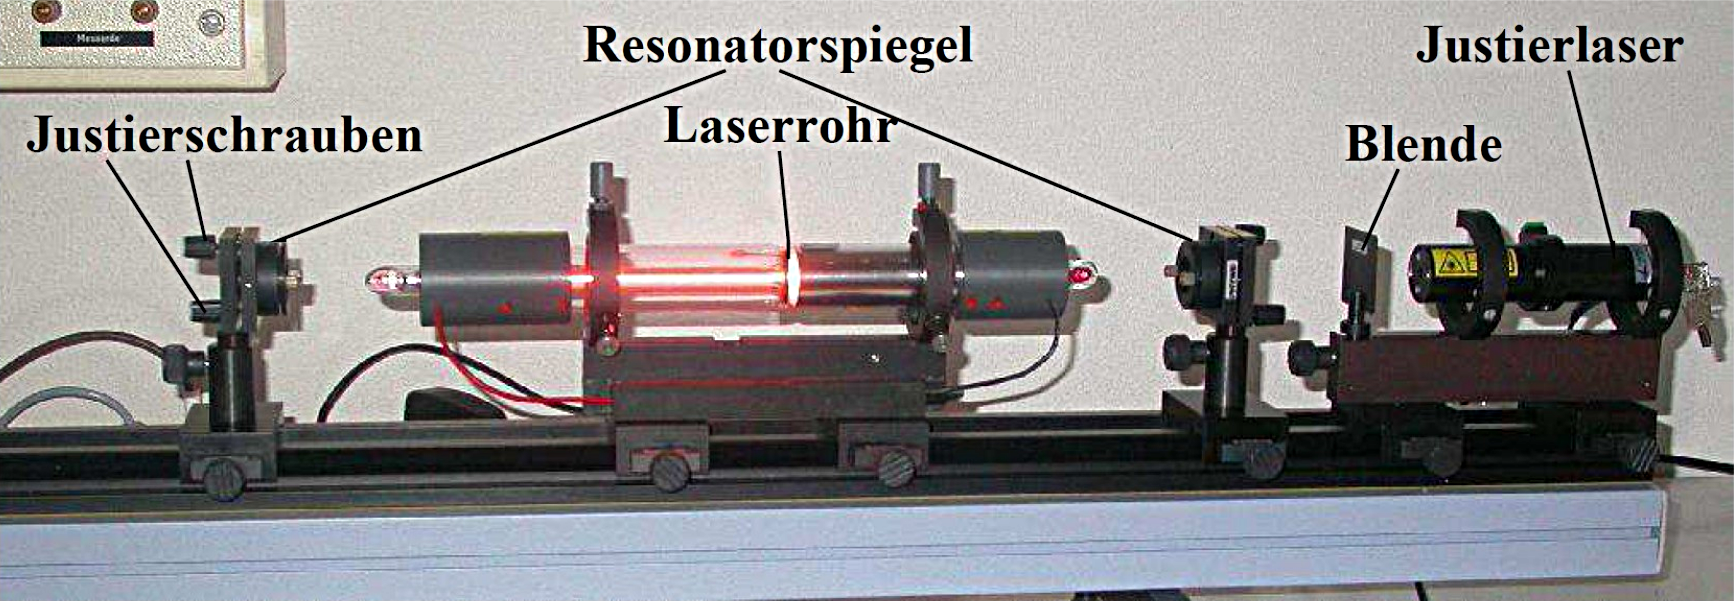
\includegraphics[width=0.8\textwidth]{images/aufbau.png}
  \caption{Seitenansicht des Grundaufbaus \cite{anleitung}.}
  \label{fig:aufbau}
\end{figure}


\section{Durchführung}
\label{sec:durchfuehrung}
In der ersten Messaufgabe wird der Laser in Betrieb genommen.
Dafür werden mit dem Justierlaser die Spiegel so eingestellt,
dass die Reflexionen in einem Punkt auf die Blende vor dem Justierlaser treffen.
Der linke Spiegel aus Abbildung \ref{fig:aufbau} wird erst auf der rechten Seite zwischen Laserrohr und Blende montiert.
Wenn die Spiegel korrekt justiert sind, kann der Laser in Betrieb genommen werden.
Es wird für die Kombination aus zwei konkaven und einem konkaven und planaren Spiegel die
Abhängigkeit der Intensität von der Resonatorlänge mit eine Photodiode aufgenommen.

Die Modenmessung erfolgt mithilfe der Streulinse, die hinter dem Auskopplungsspiegel eingestzt wird.
Von den Moden wird auf einer horizontalen Linie die Intensität mit der Photodiode gemessen.
Um die $\text{TEM}_{10}$ messen zu k\"nnen wird ein dünner Draht in den Strahl gebracht.

Die Polarisation die durch die Brewsterfenster geschieht wird mit der Polarisationsmessung
nachgewiesen. Es wird hinter dem Resonator ein Polarisator montiert und wieder mit der Photodiode
die Intensität in Abhängigkeit des eingestellten Winkels gemessen.

In der letzten Messung werden zwei Gitter verwendet um die Wellenlänge des Lasers zu bestimmen.
Die Gitter haben $\num{80}$ und $\SI{100}{Linien\per\milli\meter}$.
Der Schirm hat einen Abstand von $\SI{134}{\centi\meter}$ zu der Position der Gitter.
